%%%%%%%%%%%%%%%%%%%%%%%%%%%%%%%%%%%%%%%%%%%%%%%%%%%%%%%%%%%%%%%%%%%%%%%%%%%%%%%%
%2345678901234567890123456789012345678901234567890123456789012345678901234567890
%        1         2         3         4         5         6         7         8

\documentclass[letterpaper, 10 pt, conference]{ieeeconf}  % Comment this line out if you need a4paper

%\documentclass[a4paper, 10pt, conference]{ieeeconf}      % Use this line for a4 paper

\IEEEoverridecommandlockouts                              % This command is only needed if 
                                                          % you want to use the \thanks command

\overrideIEEEmargins                                      % Needed to meet printer requirements.

% See the \addtolength command later in the file to balance the column lengths
% on the last page of the document

% The following packages can be found on http:\\www.ctan.org
%\usepackage{graphics} % for pdf, bitmapped graphics files
%\usepackage{epsfig} % for postscript graphics files
%\usepackage{mathptmx} % assumes new font selection scheme installed
%\usepackage{times} % assumes new font selection scheme installed
\usepackage{amsmath} % assumes amsmath package installed
%\usepackage{amssymb}  % assumes amsmath package installed

\usepackage{graphicx}


\title{\LARGE \bf
Particle Filter for Skid-Steered Robot
}


\author{Rodolfo Corona%$^{1}$ 
$~$and Joydeep Biswas%$^{2}$% <-this % stops a space
%\thanks{*This work was not supported by any organization}% <-this % stops a space
%\thanks{$^{1}$Albert Author is with Faculty of Electrical Engineering, Mathematics and Computer Science,
%        University of Twente, 7500 AE Enschede, The Netherlands
%        {\tt\small albert.author@papercept.net}}%
%\thanks{$^{2}$Bernard D. Researcheris with the Department of Electrical Engineering, Wright State University,
%        Dayton, OH 45435, USA
%        {\tt\small b.d.researcher@ieee.org}}%
}


\begin{document}



\maketitle
\thispagestyle{empty}
\pagestyle{empty}


%%%%%%%%%%%%%%%%%%%%%%%%%%%%%%%%%%%%%%%%%%%%%%%%%%%%%%%%%%%%%%%%%%%%%%%%%%%%%%%%
\begin{abstract}

The ability to determine the location of a robot in its environment is a key requirement of autonomous robotics tasks. The particle filter algorithm, which may be used with various different combinations of sensors, is a common approach to this problem. Through the development of effective motion models for a skid-steered, outdoor robot, we have implemented a particle filter which may be used to test the effectiveness of a variety of sensors. Having tested the algorithm with a combination of odometry and GPS, we will explore methods from computer vision, such as convolutional neural networks (CNNs), for effectively incorporating video cameras as sensors. To this end, we have collected a data set of images mapped to locations on a variety of maps which vary in size and path complexity, something which will allow us to test both the efficacy and robustness of the methods we will explore.

\end{abstract}


%%%%%%%%%%%%%%%%%%%%%%%%%%%%%%%%%%%%%%%%%%%%%%%%%%%%%%%%%%%%%%%%%%%%%%%%%%%%%%%%
\section{INTRODUCTION}
For an autonomous robot to operate effectively in its environment, it is necessary that it be able to track its location over time. More formally, \textbf{localization} may be defined as the task of determining a robot's \textbf{pose}, which is of the form $(x~y~\theta)^T$ and denotes a robots location and orientation within a given map $M$. Although, simple to define, this task is made difficult by the inherently noisy nature of sensors. Even if a particular sensor's error is small, the dependence of each reading on the previous ones can quickly give rise to large systematic errors.  
\par
In order to combat this problem, localization algorithms often require and are greatly aided by the use of multiple sensors. By getting location estimates from a variety of sources, a tighter probability distribution for a robot's pose may be computed, allowing the error and uncertainty in pose estimates to be mitigated. 
\par
In this paper we detail the implementation of a \textbf{particle filter}, a popular localization algorithm, for use with the Jackal, a skid-steered, outdoor robot developed by ClearPath Robotics\footnote{https://www.clearpathrobotics.com/jackal-small-unmanned-ground-vehicle/}. To this end, we derive a motion model for the robot and employ the use of GPS sensors as well as its internal odometry for our implementation.

\begin{figure}[h]
\centering
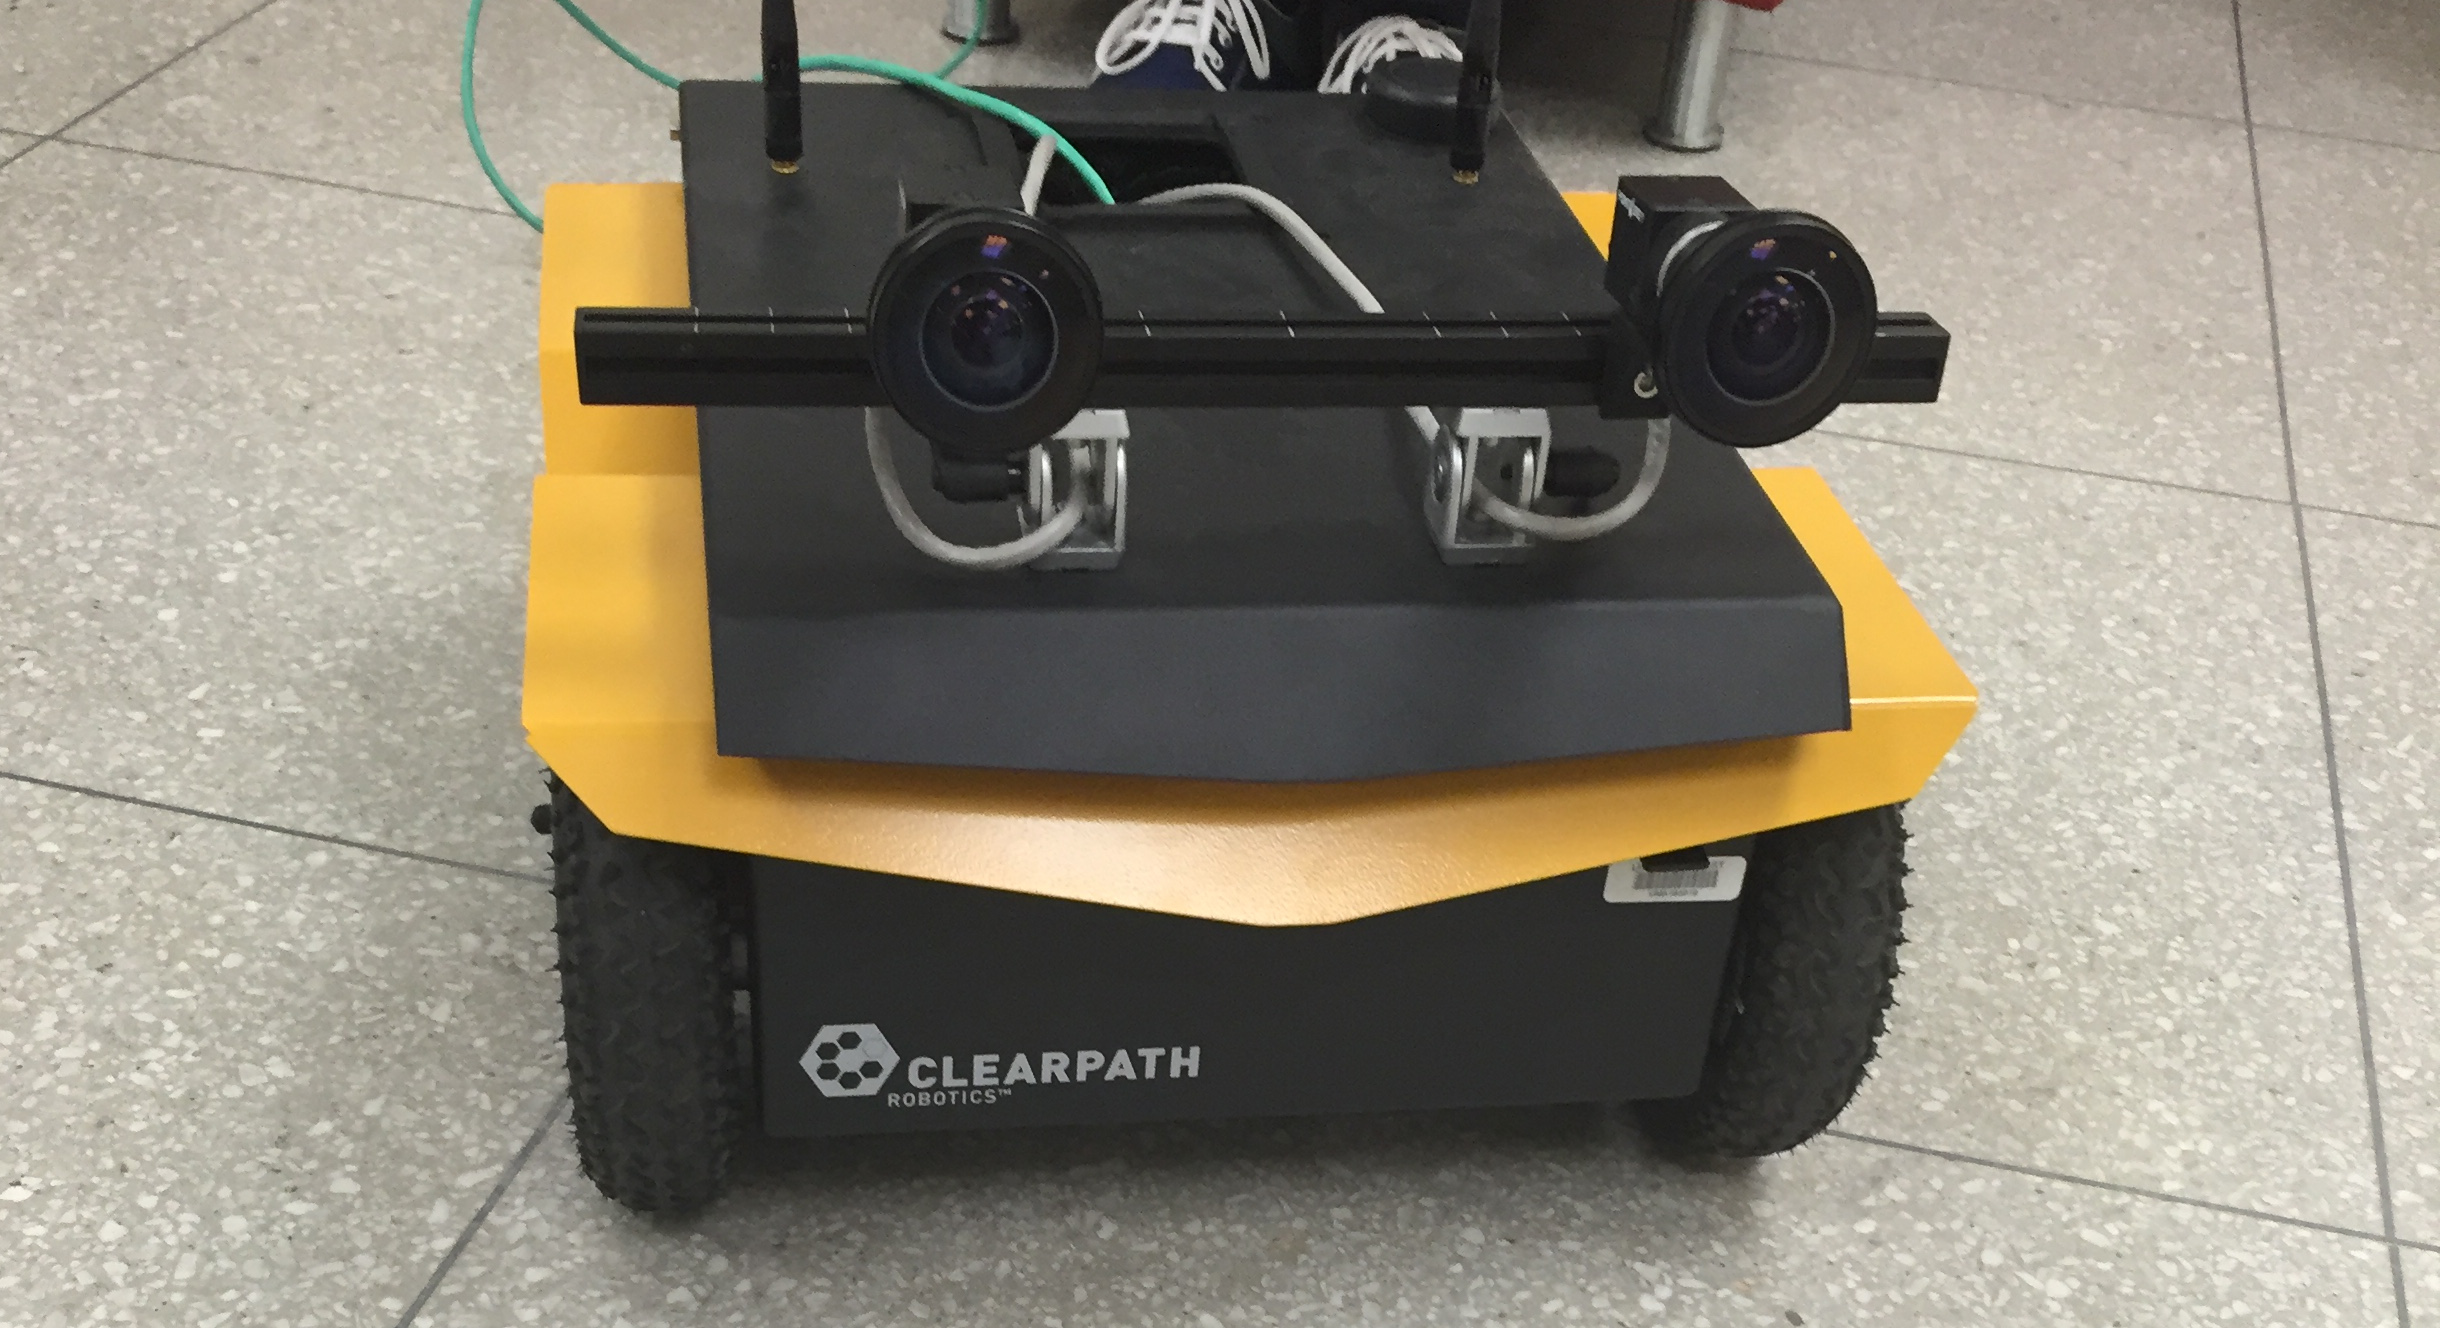
\includegraphics[scale=0.09]{jackal}
\caption{The ClearPath Jackal equipped with two fish-eye camera lenses.}
\end{figure}

\par 
This work also explores how cameras may be used as sensors for localization. In order to map images to pose estimates, we use convolutional neural networks (CNNs) to extract high-level feature vectors from images, which are then experimented with using a variety of different classification algorithms. 

\section{Background}
\subsection{Localization}
The task of any localization algorithm is to determine a likely estimate for a robot's current pose $(x~y~\theta)^T$. In order to accomplish this, the algorithm must work effectively with readings from its ensemble of sensors. 
\par
At each time step $t$, a robot receives a \textbf{control} $u_t$, and a \textbf{sensor reading} $z_t$. The control is an estimate of the robot's translation and rotation since the last time step as given by its internal sensors, such as odometry and IMU (inertial measurement unit), and is of the form $(\Delta x~\Delta y~\Delta \theta)^T$. Similarly, the sensor readings come from sensors external to the robot, such as GPS or laser range finders, and give a pose estimate of the form $(x_z~y_z~\theta _z)^T$. 
\par 
Using these readings, the robot's most likely pose $\textbf{x}_t=(x_t~y_t~\theta _t)^T$ may be found using the following formula: 
$$
\textbf{x}_t = argmax_{\textbf{x}}~P(\textbf{x}|\textbf{x}_{0:t-1}, u_{0:t}, z_{0:t})
$$
Given that the space of possible poses is continuous, however, makes the task of searching through it intractable. Further, the cost of computing such a function can quickly grow too large because of the dependence of the estimate on all previous estimates and readings. 
\par
In order to combat the growth of the cost, the \textbf{Markov assumption} may be used, allowing us to compute an estimate using only the current time step's readings and the previous time step's pose estimate:
$$
\textbf{x}_t = argmax_{\textbf{x}}~P(\textbf{x}|\textbf{x}_{t-1}, u_t, z_t)
$$
\par
For working tractably in a continuous space, localization algorithms use a variety of methods to approach this function. The most common strategy is to assume that the control and sensor readings are independent from each other and split the function into two statistical models, the \textbf{motion model} and the \textbf{perceptual model}. The motion model approximates the probability distribution $P(\textbf{x}_t|\textbf{x}_{t-1},u_t)$ using the control reading and noise generated from experimentally derived distributions such as Gaussians. The perceptual model approximates the probability distribution $P(\textbf{x}_t|z_t)$ using experimentally derived distributions to model sensor uncertainty. In general, the motion model is used in order to estimate the trajectory of the robot over time. Given the dependence of each motion model estimate on the previous time step's estimate, the motion model is highly prone to systematic errors. The perceptual model is therefore used in order to bias this trajectory estimate and keep the error in check. 

\subsection{Particle Filters}

The approach of the particle filter algorithm to the problem of tractability is to use a discrete set of $N$ random variables known as \textbf{particles}. At each time step, particles are assigned different pose estimates based on the robot's models. This distribution of particles is then used in order to approximate the true probability distribution of the robot's pose. 
\par
To accomplish this, the algorithm iterates through three main procedures at each time step. Firstly, each particle's pose estimate is computed using its previous pose and the current control readings in the \textit{elapse time} step. Following this, the \textit{weighing} step uses the current sensor reading in order to assign weights to each particle's estimate. Finally, in the \textit{resampling} step, a probability distribution of possible poses is computed based on the particle poses and weights, which is used to re-sample the particles' poses. 

\subsubsection{Elapse Time}
At each time step $t$ the robot's motion model is used in conjunction with the current control reading $u_t$ in order to derive a new pose for each particle:
\begin{align*}
\textbf{x}_t = \begin{bmatrix}
				x_t \\
				y_t \\
				\theta _t
				\end{bmatrix} 
				=
				\begin{bmatrix}
				x_{t-1} + x_u + \epsilon _x\\
				y_{t-1} + y_u + \epsilon _y\\
				\theta _{t-1} + \theta _u + \epsilon _\theta				
				\end{bmatrix}
\end{align*}
Where $\epsilon$ represents an error reading sampled from an experimentally approximated distribution for each of the three dimensions. 
\subsubsection{Weigh}
Immediately after receiving a pose estimate, each particle is assigned a weight based on the current sensor model reading $z_t$. In order to effectively use GPS for localization, the latitudinal and longitudinal variances, $\sigma _{lon}^2$ and $\sigma _{lat}^2$, for the Jackal's GPS were approximated experimentally by collecting readings from a set of three marked places five different times. Using these values, the following loss function was constructed:
$$
f(x_e,y_e,x_g,y_g)= \frac{1}{\sigma _{long}^2 + e^{|x_e-x_g|}}\cdot \frac{1}{\sigma _{lat}^2 + e^{|y_e-y_g|}}
$$
Where $x_e$ and $y_e$ are position estimates and $g_x$ and $g_y$ are GPS position readings. This function is then used in order to assign a weight to each particle, where a greater distance from the GPS reading results in a lower weight being assigned. 
\subsubsection{Resample} 
Using each of the $N$ particles' weight, a discrete probability density function of pose estimates is built such that the probability of any particle's pose estimate is proportional to its weight: 
$$
\forall _{1\leq i \leq N}~P(\textbf{x}^i)=\frac{w_i}{\sum _{i=1} ^N w_i}
$$
Where $\textbf{x}^i$ and $w_i$ denote the $i$-th particle's pose estimate and weight. Each particle's pose estimate is then re-sampled using this distribution, which results in the particle distribution being concentrated around the most likely robot locations.  

\begin{figure}[h]
\centering
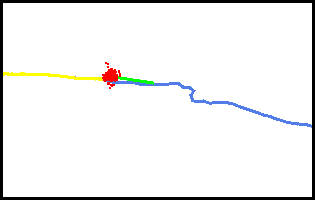
\includegraphics[scale=0.70]{particle_filter_visual}
\caption{A visualization of the particle filter using GPS. The blue path denotes the set of all GPS readings while the yellow path denotes the readings already given to the robot. The red dots represent the particle distribution and the green line, stemming from the particle cloud, represents the robot's pose.}
\end{figure}

\section{Methodology}

\subsection{Data Set}
A roughly 280 meter path was chosen for use as a map for testing our particle filter. This path was traversed a total of 19 times at different times of day in order to capture as much variability in daylight as possible. Through each run, data from all robot sensors was collected (e.g. GPS, cameras, etc.).  

\begin{figure}[h]
\centering
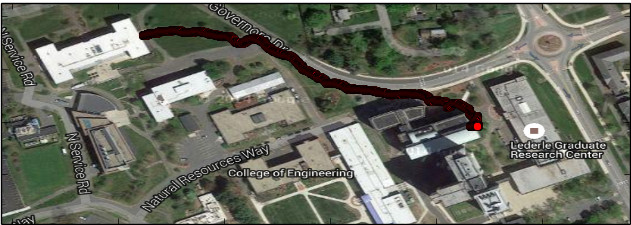
\includegraphics[scale=0.5]{map}
\caption{A satellite image of the map used in our data set. The red map shows the path traversed by the robot during data collection.}
\end{figure}

\subsection{Neural Perceptual Model}
In order to effectively use cameras as sensors, a method that can work directly with raw RGB information with as little preprocessing as possible is desirable. CNNs are a well known tool that has been previously used with raw image data for a variety of machine learning tasks, particularly in object recognition. 
\par
Through a series of convolution operations on the image data, CNNs are able to extract higher level features from images such as edges and partial objects, features which we believe will prove effective in differentiating pictures taken at different locations from each other. 
\par
To this end, a pre-trained model of the AlexNet CNN architecture, which won the 2012 ImageNet Large Scale Visual Recognition Competition (ILSVRC), is used in order to extract higher level features from the images in our data set. Rather than use the entire network for our classification task, these feature vectors are used with a variety of different classification algorithms (e.g K-Nearest Neighbors, SVNs, etc.) in order to determine an effective model for localization.  

\addtolength{\textheight}{-12cm}   % This command serves to balance the column lengths
                                  % on the last page of the document manually. It shortens
                                  % the textheight of the last page by a suitable amount.
                                  % This command does not take effect until the next page
                                  % so it should come on the page before the last. Make
                                  % sure that you do not shorten the textheight too much.

%%%%%%%%%%%%%%%%%%%%%%%%%%%%%%%%%%%%%%%%%%%%%%%%%%%%%%%%%%%%%%%%%%%%%%%%%%%%%%%%



%%%%%%%%%%%%%%%%%%%%%%%%%%%%%%%%%%%%%%%%%%%%%%%%%%%%%%%%%%%%%%%%%%%%%%%%%%%%%%%%



%%%%%%%%%%%%%%%%%%%%%%%%%%%%%%%%%%%%%%%%%%%%%%%%%%%%%%%%%%%%%%%%%%%%%%%%%%%%%%%%




\end{document}
